\chapter{Karst and karstification process}
\section{Introduction}
%Formation of karst caves is inherently connected with the karst
This chapter will briefly describe karst and processes that govern the
development of karts caves. First, basic definitions are introduced followed by
description of elements of karst landscape and formations. Next, a high level
overview of the karstification process is presented along chemical reactions
in limestone aquifers that are essential in formation of caves. Process and
chemistry of speleothem formation is described at the end of the chapter.
\section{Basics}

\subsection{Definitions}
\begin{description}
  \item[Karstification]
    not a strictly defined term. Depending on context it may
    mean all forms of corrosion of soluble rocks or it may encompass whole range of
    processes that lead to devolopment of karst formations.
    
    Usually karstification means a landscape forming process that consists of dissolution
    of various kinds of bedrock. The most common kinds of solutes are limestone,
    dolomite, and gypsum \parencite{karstglossary}. However, given right conditions
    even some weathering-resistant rocks like quartzite may be subject to 
    karstification \parencite{migon2010}\todo{Check reference}.
    
    Although chemical dissolution is the main driving force behind karstification,
    mechanical forces may also play a role in the final looks of the karst landscape.
    That's why sometimes, all these forces together are put under the umbrella term
    of karstification.

  \item[Karst]
    terrain formation developed throught the means of
    \emph{karstification}. The origin of the term is a German form of Slavic word
    kras or krš meaning bleak, waterless place \parencite{karstglossary}.
  \item[Karst cave]
    hollow space in a karst structure that is large enough for human to enter
    \parencite{hill1997cave}
  \item[Aquifer]
    geological formation that is capable of holding large amounts of water
    through porosity, and other empty spaces inside.
  \item[Recharge]
    process of addition of water to an aquifer.
\end{description}
\subsection{Elements of karst landscape}

\begin{figure}
  \centerline{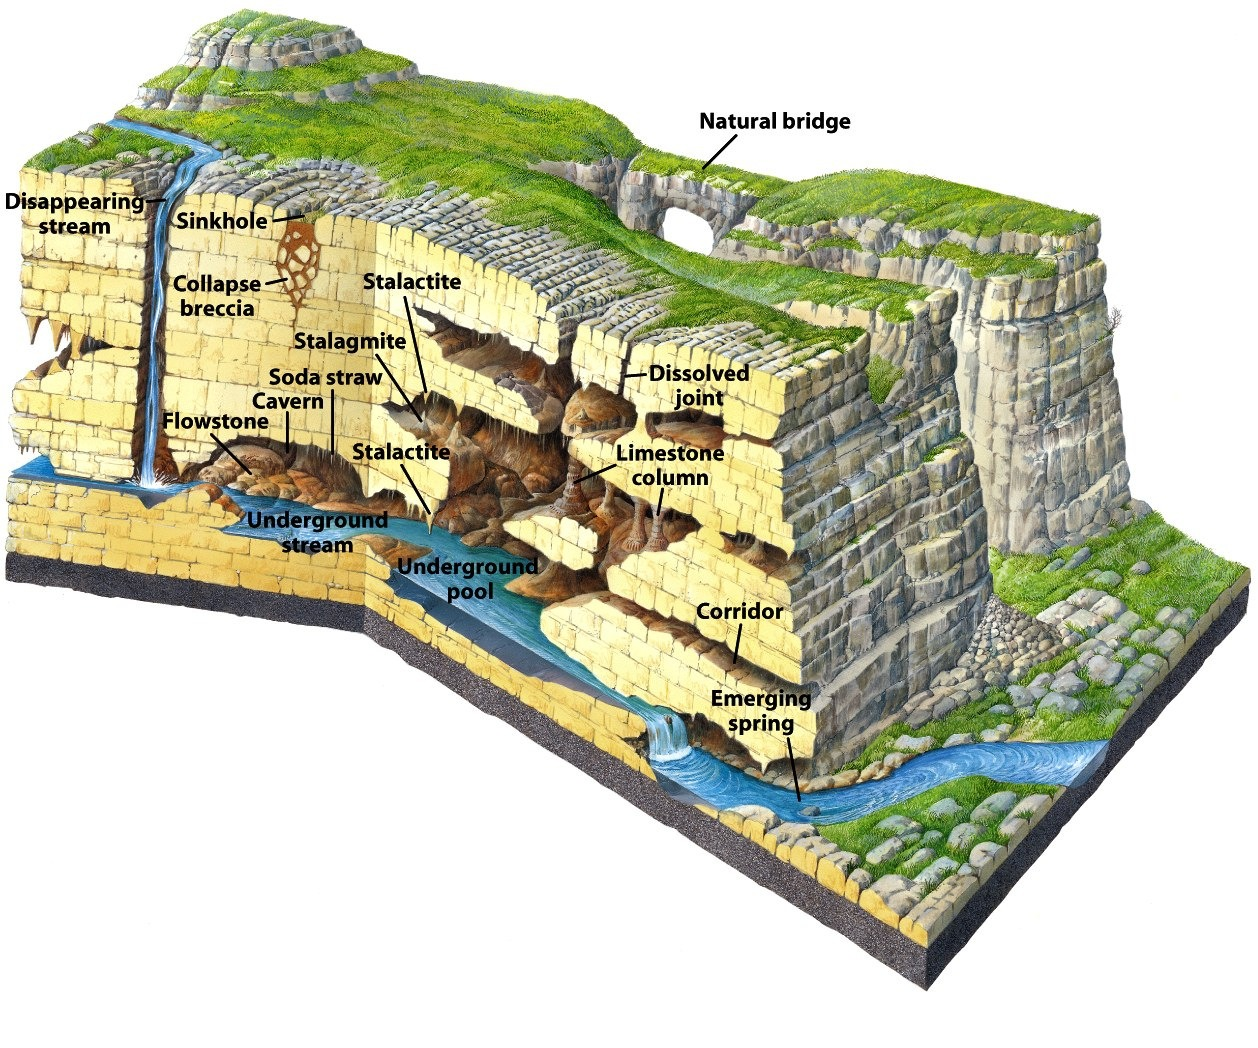
\includegraphics[width=\textwidth]{chapters/karstification/karst_landscape.jpg}}
  \caption{Karst landscape showing various features of karst aquifers.
    Figure from book by \cite{marshak2006}}
  \label{fig:karstlandscape}
\end{figure}


Karstification process may produce very interesting and varied landscape. Some
of the prominent elements of karst landscapes seen in figure \ref{fig:karstlandscape}
are:

\begin{description}
  \item[Sinkholes]
  \item[Caves]
  \item[Resurgences]
    places where water that went into the aquifer is reemerging to the surface
  \item[Disappearing streams]
  \item[Tunnels]
  \item[Shafts]
\end{description}
\todo{describe each formation}

\section{Overview of the karstification process}

The most important factor in karstification process is flow of solvent throught an
underground aquifer. Since bedrock is subject to geological processes, a
net (sometimes called a matrix) of fractures of varying diameter and shape is
present in it. This solvent, usually water, flows through this kind of net and
reacts with rock in ways described later.

Such karst aquifer may be surrounded on its sides by an aquitard, a substance
that is impenetrable to water.

Water that enters the system may come from precipation, rivers or lakes. Inflow
of water may happen through diffuse infiltration or point infiltration.
Diffuse infiltration happens on larger areas, covered by small fractures whereas
point infiltration requires a prominent fracture to be present in the aquifer
that can take large amounts of water from a river or lake.

Recharge water that comes to the karst aquifer from neighbouring non-karst areas
is called \emph{allogenic recharge}. For example on figure~\ref{fig:karstification}
a river flowing on the upper aquitard and entering the limestone aquifer through
the sinkhole is an allogenic recharge.

On the other hand, recharge water that flows directly to the karst area e.g. by
precipation is called an \emph{autogenic recharge}

Water that flows through the aquifer reacts chemically with walls of the
fractures widening them through dissolution. After going through the aquifer,
water reemerges at lower level through emerging springs or resurgences.

There are also cases of ground formation resulting from human activity.
Although not truly a karst process, a sinkhole that opened in 2010 in city of
Guatemala was a result of combination of loose ground made of volcanic ash and
inadequate draining system, that couldn't dissipate large amounts of water
brought by tropical storm Agatha \parencite{times2010}.

\begin{figure}
  \centerline{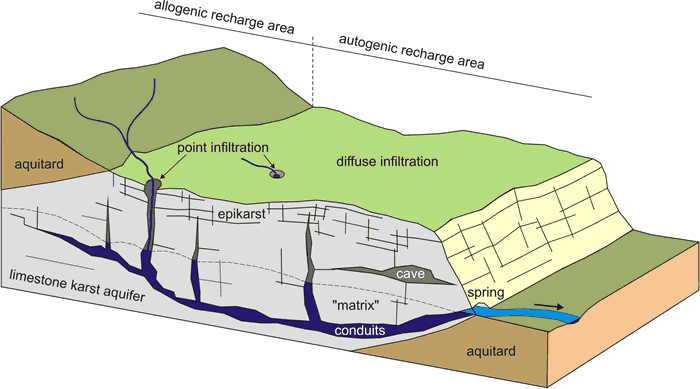
\includegraphics[width=\textwidth]{chapters/karstification/karstification.png}}
  \caption{Example of limestone karst aquifer.
    Figure from \cite{golscheider2007methods}}
  \label{fig:karstification}
\end{figure}

\section{Limestone dissolution}

Chemical reactions that take place during the karstification process will be
shown for limestone aquifers. Following description is taken form \cite{dreybrodt2002}
which is based on \cite{plummer1978}.

With the pH of solution at about 7, limestone dissolves through the following
slow reaction:

\begin{equation}
  \cee{H2O + CaCO3 <-> Ca^2 + CO3^2- + H2O}
  \label{eq1}
\end{equation}

Unfortunately, given very weak soulibility of calcium carbonate in water\footnote{Only about 0.0013~g/100~mL in 25\degree C according to \cite{aylward2008si}},
limestone dissolution would be extremely slow.

However, as the rain passes throught the atmosphere, it's picking up carbon
dioxide that gets dissolved in water. During this dissolution, small amounts of
carbonic acid are produced:

\begin{equation}
  \cee{H2O + CO2 -> H^+ + HCO3^-}
  \label{eq2}
\end{equation}

Above raction delivers a proton that bonds with carbonate detached during slow
dissolution \ref{eq1}:

\begin{equation}
  \ce{CO3^2- + H^+ -> HCO3^-}
  \label{eq3}
\end{equation}

Thanks to this, the ion activity product \ce{(CO3^2- )} \ce{(Ca^2+)} is below the
solubility constant of calcite. Calcium bicarbonate\footnote{\ce{Ca(HCO3)2}} produced
during this process has orders of magnitude better soulibility in water\footnote{16.6~g/100~mL in 20\degree C according to \cite{aylward2008si}}
what greatly enchances the rate of limestone dissolution.

\Crefrange{eq1}{eq3} can be summed up with the following single
equation:

\begin{equation}
  \ce{CaCO3 + H2O -> Ca^2+ + 2HCO3^- }
  \label{eq4}
\end{equation}

\section{Formation of speleothems}

Speleothems are mineral deposits of various kind that form in a process reverse
to dissolution. When water rich in calcium bicarbonate leaves small fissures in
the aquifer and enters big, hollow areas, its pressure lowers and causes
\ce{CO2}-degassing that is the major factor in precipation of calcium carbonate
on the surfaces of caves.

Loss of carbon dioxide leads to supersaturation in the solution reaction that
is directly reverse to reaction \ref{eq4} \parencite{fairchild2012speleothem}:

\begin{equation}
  \ce{Ca^2+ + 2HCO3 -> CaCO3 + H20 + CO2}
  \label{eq:precipation}
\end{equation}

Water evaporation plays marginal role in speleothem formation, what was shown
by \cite{holland1964cave}\todo{fix bibliography entry}.

